\documentclass{beamer}
\usepackage{setspace}
\usepackage{bm,color,float,epstopdf,amsthm,epstopdf}
\usepackage{multirow,tikz}
\newcommand{\fttheory}[1]{\fcolorbox{blue}{blue}{\color{white}\textbf{#1}\hspace{\textwidth}}}
\newcommand{\ftexampl}[1]{\fcolorbox{orange}{orange}{\color{black}\textbf{#1}\hspace{\textwidth}}}
\newcommand{\ftdata}[1]{\fcolorbox{violet}{violet}{\color{white}\textbf{#1}\hspace{\textwidth}}}
\newcommand{\ftheader}[1]{\fcolorbox{lightgray}{lightgray}{\color{black}\textbf{#1}\hspace{\textwidth}}}
\newcommand{\ftvocab}[1]{\fcolorbox{cyan}{cyan}{\color{black}\textbf{#1}\hspace{\textwidth}}}
\newcommand{\usd}{\text{ {\scriptsize USD}}}
\newcommand{\eur}{\text{ {\scriptsize EUR}}}
\newcommand{\aud}{\text{ {\scriptsize AUD}}}
\newcommand{\mxn}{\text{ {\scriptsize MXN}}}
\newcommand{\musd}{\text{ m {\scriptsize USD}}}
\newcommand{\meur}{\text{ m {\scriptsize EUR}}}
\newcommand{\maud}{\text{ m {\scriptsize AUD}}}

\renewcommand{\arraystretch}{1.5}
\begin{document}

%-----------------------------------------------------------------------------%
% application i: swaps
\begin{frame}{\ftheader{Application I: Swaps}}
	\begin{itemize}
		\item A swap is a contract in which parties ``swap'' cash-flows. 
		\item A typical contract involves one party that makes \textit{floating} payments on its debt swapping its obligations with those of another party that makes \textit{fixed} payments on its debt
		\item Swaps are portfolios of forwards. 
	\end{itemize}
\end{frame}

%-----------------------------------------------------------------------------%
% swaps: ibm and the world bank
\begin{frame}{\ftdata{Swaps: IBM and the World Bank}}
    \begin{itemize}
        \item Salomon Brothers wrote the first swap in 1981
        \item The World Bank is an international organization that borrows from developed countries and lends to developing countries
        \item In 1981, Swiss debt was cheap, so the World Bank wanted to borrow there, but...
        \item Switzerland limited how much the World Bank could borrow
        \item IBM had already borrowed in Switzerland and wanted dollars
        \item Salomon proposed ``swapping'' cash flows
        \item The World Bank borrowed dollars
        \item IBM paid the World Bank's dollar obligations
        \item The World Bank paid IBM's franc obligations
        \item It was as if the World Bank borrowed in francs and IBM borrowed in dollars
    \end{itemize}
\end{frame}

%-----------------------------------------------------------------------------%
% interest rate swaps: problem
\begin{frame}{\ftexampl{\hypertarget{frame:interestrateswaps}{Interest Rate Swaps: Problem}}}
	\textbf{Problem.} Suppose company $A$ borrowed $1\musd$ for one year at a fixed rate of 3\% and company $B$ borrowed $1\musd$ for one year at a floating rate (say the rate will either be 2\% or 4\%). Describe the forward contract that lets $A$ and $B$ swap their obligations.\\
	\vfill
	\textbf{Solution.} $A$ owes $1.03\musd$ in one year, while $B$ will owe either $1.02\musd$ or $1.04\musd$ in one year. Rather than exchange a security like a T-note, $A$ and $B$ can cash settle. So if the floating rate is 2\%, $B$ pays $A$ $.01\musd$ whereas if the floating rate is 4\%, $A$ pays $B$ $.01\musd$. By doing so, $B$ always ``owes'' $1.03\musd$ and $A$ ``owes'' $1.02\musd$ when the rate is 2\% or $1.04\musd$ when the rate if 4\%.
\end{frame}

%-----------------------------------------------------------------------------%
% application ii: exchange rates
\begin{frame}{\ftheader{Application II: Exchange Rates}}
	\begin{itemize}
		\item We're going to exam \textit{interest rate parity}, which says that you should not be able to make more money on a Euro denominated risk-free asset (e.g. German bunds) than on a Dollar denominated risk-free asset (e.g. US Treasuries) once you've accounted for spot and future prices in the foreign currency market
    \end{itemize}
\end{frame}

%-----------------------------------------------------------------------------%
% interest rate parity
\begin{frame}{\fttheory{Interest Rate Parity}}
    \begin{itemize}
        \item Two countries, domestic ($D$) and foreign ($F$), $r_{D}$ is the risk-free rate in $D$, $r_{F}$ in $F$, $E_{0}$ is the spot price of $F$'s currency, and $K_{0}$ is the price of a forward on $F$'s currency
		\item \textit{Interest Rate Parity} occurs when
            \begin{equation}
				\boxed{1+r_{D}=(1+r_{F})\cdot\frac{K_{0}}{E_{0}}}
            \end{equation}
    \end{itemize}
\end{frame}

%-----------------------------------------------------------------------------%
% interest rate parity: problem
\begin{frame}{\ftexampl{\hypertarget{frame:interestrateparity}{Interest Rate Parity: Problem}}}
	\textbf{Problem.} $1\aud$ costs $E_{0}=.64\usd$. The yields on 1-year Australian and US government bonds are $r_{F}=.245\%$ and $r_{D}=.3\%$ respectively. What should the 1-year forward price of $1\aud$ be? What should the 1-year forward price of $1\usd$ be? If the 1-year forward price of $1\aud$ is $K_{0}=.6402\usd$, what arbitrage opportunity is available to you?\\ 
\vfill
	\textbf{Solution.} Let's first compute what the forward price should be under Interest Rate Parity:
	\begin{equation}
		K_{0}=\frac{1+r_{D}}{1+r_{F}}\cdot E_{0}=\frac{1+.00300}{1+.00245}(.64\usd)=.6404\usd
	\end{equation}
	The forward price for $1\usd$ should be 
	\begin{equation}
		1\usd\:/(.6404\usd\:/\aud)=1.5615\aud
	\end{equation} 
	(You can get the same number by flipping the roles of $F$ and $D$)
\end{frame}

%-----------------------------------------------------------------------------%
% interest rate parity: problem
\begin{frame}{\ftexampl{Interest Rate Parity: Problem}}
	\textbf{Solution (continued).} The 1-year forward price of $.6402\usd$ is \textit{less} than what it should be under interest rate parity (buying AUD with USD using the forward is ``cheap''). Equivalently, the 1-year forward price of $(1/.6402)\aud=1.5620\aud$ is \textit{greater} than what it should be under interest rate parity (1 USD buys you more AUD than it should). This leads us to believe that we should borrow in AUD, invest in USD, then use the forward to get back AUD.
\end{frame}

%-----------------------------------------------------------------------------%
% interest rate parity: problem
\begin{frame}{\ftexampl{Interest Rate Parity: Problem}}
	\textbf{Solution (continued).} To exploit the arbitrage opportunity, use the following procedure.\\
	\vfill
	Today, 
	\begin{enumerate}
		\item borrow $1\maud$, 
		\item buy $1\maud\times(.64\usd\:/\aud)=.64\musd$
		\item buy $.64\musd$ of US government bonds
		\item \underline{write} a 1-year forward for $1.5620\aud\:/\usd$
	\end{enumerate}
	In one year, 
	\begin{enumerate}
		\item collect $(1+.003)\times(.64\musd)=.6419\musd$
		\item $.6419\musd\times(1.5620\aud\:/\usd)=1.0027\maud$
		\item repay $1\maud\times(1+.00245)=1.0025\maud$ 
		\item you have collected a profit of $.0002\maud$ (about $200\aud$)
	\end{enumerate}
\end{frame}

%-----------------------------------------------------------------------------%
% irp vs. ppp
\begin{frame}{\ftexampl{Interest Rate Parity vs. Purchasing Power Parity}}
	\begin{itemize}
		\item Can we apply the same logic to other assets?
		\item \textit{Purchasing power parity} refers to the ability to buy the same basket of goods/services around the world for the same price
        \item A taco in the US sells for $3\usd$, a taco in Mexico sells for $20\mxn$, a peso sells for $.05\usd$. What arbitrage opportunity is available to you?
        \item Buy $20\mxn$ for $1\usd$, buy 1 taco in Mexico for 20$\mxn$, sell 1 taco in the US for $3\usd$. You've made $2\usd$.
		\item Money can be moved around the world (almost) costlessly. Tacos cannot.
    \end{itemize}
\end{frame}

%-----------------------------------------------------------------------------%
% the economist's big-mac index
% TODO: eventually, I'd like to do bigmac on one side, interest rates on other
\begin{frame}{\ftdata{The Economist's Big-Mac Index}}
    \begin{center}
        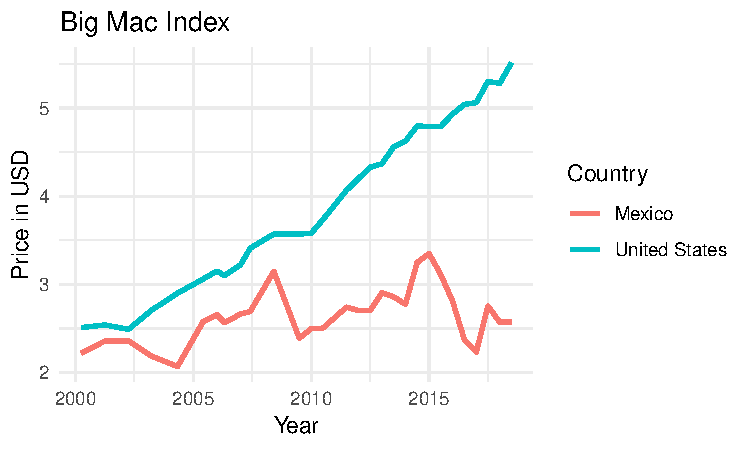
\includegraphics[scale=.75]{bigmac}
    \end{center}
	\noindent Although interest rate partity tends to hold in the data, does not. This is call the Penn effect and it is due to (1) limits to arbitrage and (2) differences in economic development. \\
\end{frame}

\begin{frame}{\ftexampl{Problems}}
	\begin{enumerate}
		\item \hyperlink{frame:payoffs1}{Forward Payoffs: Problem 1}
		\item \hyperlink{frame:spotfuturesparityhedging}{Spot-Futures Parity: Hedging Problem}
		\item \hyperlink{frame:spotfuturesparitymargin}{Spot-Futures Parity: Margin Problem}
		\item \hyperlink{frame:pricingexistingforwards1}{Pricing Existing Forwards: Problem 1}
		\item \hyperlink{frame:pricingexistingforwards2}{Pricing Existing Forwards: Problem 2}
		\item \hyperlink{frame:interestrateswaps}{Interest Rate Swaps: Problem}
		\item \hyperlink{frame:interestrateparity}{Interest Rate Parity: Problem}
	\end{enumerate}
\end{frame}
\end{document}
